\section{Theoretische Grundlagen}
\subsection{Definition von Halbleitern}
Insgesamt werden Materialien mit elektrischer Leitfähigkeit in drei Kategorien aufgeteilt. Der unterschied liegt im spezifischen Widerstand $\rho$.
Dieser über die Fläche $A$ die Länge $l$ so wie den Ohmschen Widerstand $R$ definiert.
\begin{equation}
	\rho=R\cdot\frac{A}{l}
	\label{SpezifischesR}
\end{equation}
Wenn für den spezifische Widerstand ($\rho\geq10^8\,\Omega$cm) ist handelt es sich um einen Isolator. Für einen Leiter muss ($\rho\leq10^3\,\Omega$cm) gelten. Im Bereich dazwischen handelt es sich um Halbleiter. Halbleiter sind sehr Temperatur abhängig so werden bei höheren Temperaturen mehr Elektronen frei was die Leitfähigkeit erhöht. 
\subsection{Bändermodell}
Für ein besseres Verständnis von Halbleitern wird das Bändermodell genutzt. Dieses kann man Quantenmechanisch oder durch Wechselwirkungen herleiten.\par 
Wenn man sich ein einzelnes Atom anschaut haben sind Elektronen auf diskrete  Energieniveaus verteilt. Wenn man nun mehrere Atome nahe zusammen bringt Wechselwirken die Elektronen miteinander. Dass heißt die Wellenfunktionen überschneiden sich und es entstehen mehrere leicht von einander getrennte Energieniveaus aufgrund des Pauliprinzips. Bei einer hohen Anzahl von Atomen werden aus diesen Einzelnen Niveaus sogenannte Energiebänder aus den ganzen einzelnen Niveaus.
Abbildung \ref{WW} zeigt dies noch einmal Grafisch.\par
\begin{figure}[ht]
	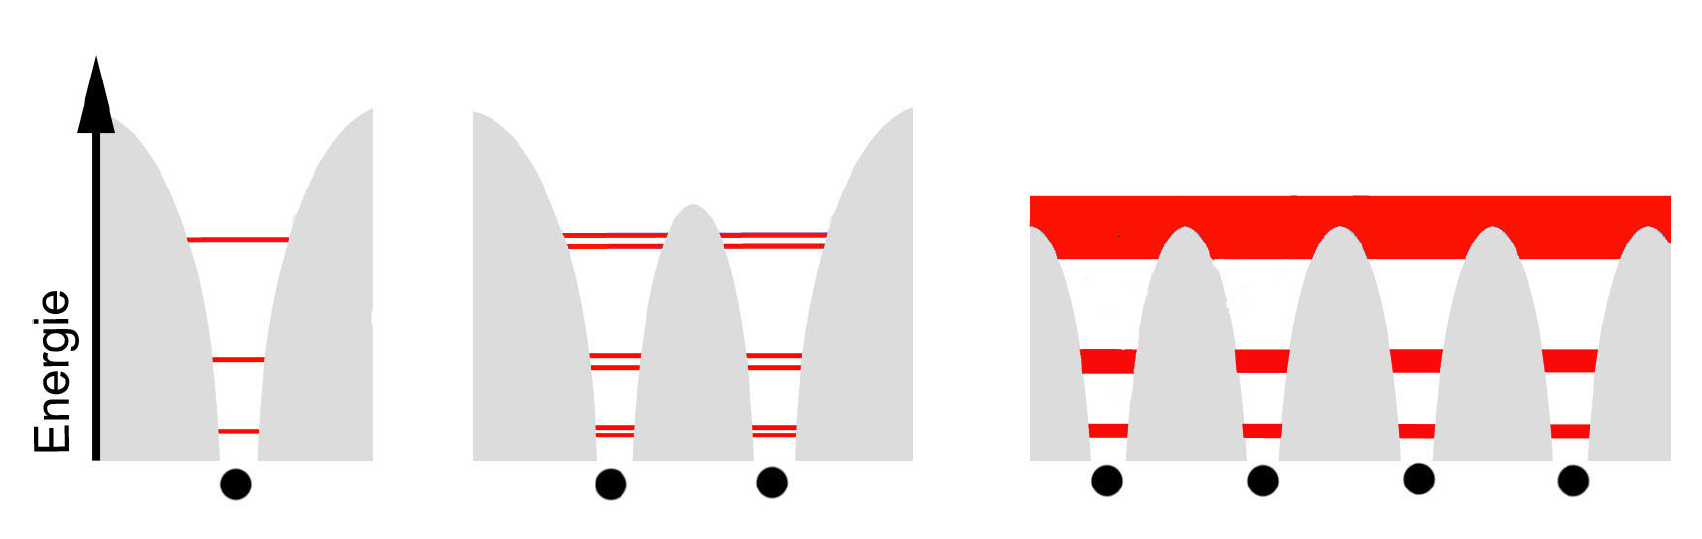
\includegraphics[scale=0.4]{Bild/Bendermodel}
	\centering
	\caption[Bändermodel]{Energieniveaus der Atome in rot. Ganz links die Energieniveaus eines einzelnen Atoms. In der Mitte die die Niveaus von zwei Atomen. Rechts die erzeugt die Wechselwirkung von mehreren Elektronen erzeugt zusätzliche Energieniveaus und damit die Energiebänder.}
	\label{WW}
\end{figure}
Eine Eigenschaften dieser Bänder ist, dass sie bei niedrigerem Energieniveau kleiner werden da die Elektronen stärker an den Kern gebunden sind. Die Breite hängt aber weiterhin von der nähe der Atomrümpfe ab. Bei einer Gitterkonstante der Atome die klein genug ist kann die Wechselwirkung sogar die Feinstruktur überwinden. Z.B kann man in Silizium ab einem gewissen Punkt nicht mehr von s oder p-Orbitalen sprechen kann. Diese werden in so einem Fall zu $sp^3$-Hybridorbital zusammengefasst.\par
Von besonderem Interesse sind zwei Bänder einmal das Valenzband welches die höchste Energie besitzt und bei $0$\,K voll besetzt ist und damit nicht mehr zum Leitfähigkeit beiträgt da sich die Elektronen Impulse alle auslöschen.\par
Das andere wichtige Band ist das Leitungsband. Dieses liegt über dem Valenzband (Energetisch gesehen). Hier sind Elektronen die zur Leitfähigkeit beitragen können da ihr Impuls bei einer Spannung nicht zu Null wird. D.h bei Material mit Elektronen im Leitungsband kann ein Strom fließen.\par
Wenn man nun sich die Definitionen von Leitern, Halbleitern und Isolatoren anschaut wird klar, dass Isolatoren bei $0\,$K ein voll besetztes Valenzband haben und keine Elektronen im Leitungsband. Ganz im Gegensatz zu Leitern bei dehnen sich die beiden Bänder überschneiden so dass ein Strom ohne zusätzlichen Energie aufwand von Valenz in das Leitungsband wechseln können. Wenn man jetzt Halbleiter bei $0$\,K betrachtet ist klar haben diese auch ein Vollbesetztes Valenzband jedoch ist der Abstand zwischen Valenzband und Leitungsband $E_g$ klein genug $(E_g\approx1\,)$eV um durch thermische Anregung Elektronen in das Leitungsband zulassen. Dies ist bei Isolatoren Theoretisch auch möglich jedoch wegen dem hohen Abstand unwahrscheinlich.\par
Auf den Quantenmechanischen Ansatz wird hier nicht weiter eingegangen. Eine genaue Erklärung ist jedoch im Staatsexamen zu Halbleitern und Halbleiter Detektoren von Simon Amrein.  \cite{Staatsexamen}\\
\subsection{Quasi freie Ladungen und Löcher}
Das Bändermodel kann nun genutzt werden um die Ladungsträger die bei Halbleitern durch das anlegen einer Spannung fließen. Sollte bei einem Halbleiter kein Elektron im Leitungsband sein wird zu beginn durch das Anlegen einer Spannung kein Strom fließen, erst wenn einem Elektron im Valenzband genug Energie zugeführt wird, dass es in Leitungsband übergeht kann es sich bewegen. Jedoch ist dieses Elektron nur Quasi frei da es sich nicht frei sondern nur in einem Periodischen Potenzial bewegen kann.\par
Eine andere Möglichkeit die Ladungsübertragung zu sehen ist mit der Hilfe von Defektelektronen oder Löchern. Wenn ein Elektron durch die Spannung abgesaugt wird hinterlässt es ein Loch. Dieses Loch kann als Positive Ladung gesehen werden. Wenn nun ein anderes Elektron dieses Loch füllt hinterlässt es seinerseits ein Loch. Dadurch wandert das Defektelektron in die entgegengesetzte Richtung zu den Elektronen als ein gedachter Positiver Ladungsträger.
\subsection{Arten von Halbleitern}
Halbleiter können in verschiedene Klassen aufgeteilt werden.\par
\subsubsection{Elementare und Verbindungshalbleiter}
Ein Elementarer Halbleiter ist ein Halbleiter welcher nur aus einem einzigen Material erstellt wurde. Silizium ist hierfür ein klassisches Beispiel. Es gibt aber neben diesen auch Verbindungshalbleiter welche aus mindestens zwei Materialien erstellt wurde. Hierbei ergänzen sich die Materialien so, dass sie die selbe Struktur wie ein elementarer Halbleiter bilden.
\subsubsection{Direkte und Indirekte Halbleiter}
Bei dieser Unterteilung wird ein weiterer Faktor betrachtet. Bisher wurden die Bänder nur in der Form von Energieniveaus betrachtet. Jedoch kann man das ganze auch im Impulsraum darstellen. Abbildung \ref{Indirekt} stellt hier den Unterschied im Impulsraum dar. Wenn wie auf der rechten Seite der Abbildung das Maxima des Valenzbandes und das Minima des Leitungsbandes übereinander liegen haben wir einen direkten Halbleiter bei dem der Impuls keine Rolle spielt. Auf der linken Seite ist dies jedoch nicht der Fall. D.h wir haben einen indirekten Halbleiter bei dem zusätzlich noch ein Impuls $\Delta p$ benötigt wird.
\begin{figure}[ht]
	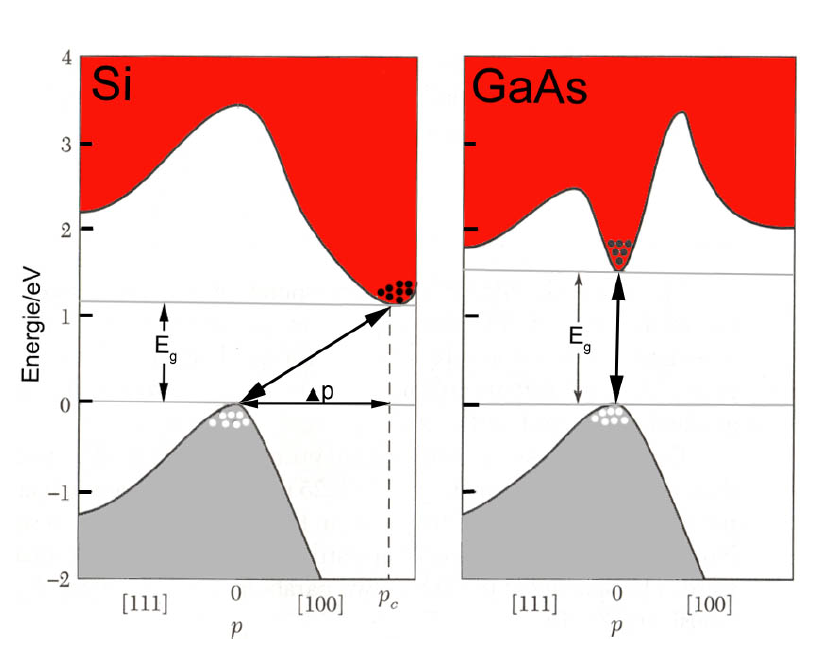
\includegraphics[scale=0.6]{Bild/InDi}
	\centering
	\caption[Indirekt und Direkte Halbleiter]{Links ein Indirekter Halbleiter im Impulsraum bei dem neben der Bandlückenenergie $E_g$ noch ein Impuls $\Delta p$. Rechts ein Direkter Halbleiter im Impulsraum der keinen Impuls benötigt.}
	\label{Indirekt}
\end{figure}
\subsubsection{Intrinsisch und Extrinsisch Halbleiter}
Intrinsische Halbleiter sind frei von Unreinheiten durch andere Stoffe und keine Fehler in der Gitterstruktur. Dass heißt sie kommen in der Realität nicht vor. Echte Halbleiter sind Extrinsische Halbleiter und haben Unreinheiten. Dies kann zu ungewollten Energieniveaus und damit anderen Eigenschaften führen. So kann z.B ein Extrinsischer Halbleiter aus Atomen mit vier Bindungen bestehen. Wenn nun ein anderes Atom in der Struktur ist mit nur drei oder fünf Elektronenbindungen bleibt ein Elektron ungebunden oder es entsteht ein Loch. Diese Unreinheiten sind meistens ungewollt können aber auch gewollt sein. Dies nennt man dann Dotierung also ein künstliches erzeugen von quasi freien Elektronen oder Löchern.
\subsection{p-n-Dioden}
Allgemein wird Dotierung in zwei Typen aufgeteilt. In n und p Dotierung. Bei der p-Dotierung werden Atome in das Gitter implantiert welche als Elektronen Akzeptoren dienen wodurch ein Elektronenüberschuss entsteht. Bei einer n-Dotierung werden Elektronen Donatoren eingesetzt welche Löcher verursachen. Dieses hinzufügen von von freien Elektronen oder Löchern wirkt sich positiv auf die Leitfähigkeit des Halbleiters aus.\par
Diese Dotierungen werden bei dem Bau von p-n-Dioden verwendet. Hierbei werden zwei Halbleiter, ein p und ein n Dotierter, aneinander gesetzt. An der Grenze diffundieren die Elektronen aus der p-Type-Schicht in die n-Type-Schicht. Die freien Ladungen löschen sich also in diesem Bereich aus. Die weiter von einander getrennten Ladungen können dies nicht machen da die Atome in ein Gitterstruktur eingebunden sind. Dies sorgt dafür dass sich ein Elektrisches Feld im Kontaktbereich ausbildet. Die dabei entstehende Spannung wird Kontakt Potential $U_{bi}$ genannt.  
